\documentclass{beamer}[14pt]
\usetheme{Copenhagen}
\usecolortheme{seahorse}
%good themes
% Copenhagen
% Darmstadt
% CambridgeUS
% boxes
%good color themes
% seahorse
\beamertemplatenavigationsymbolsempty
\usepackage{tikz}
\usepackage{tkz-graph}
\usepackage{pgfplots}
\usepackage{xcolor}
\usepackage{algorithm}


\begin{document}
	\title{Presentation 1}
	\author{Fynn Lohren, Carsten Schubert, Leon Suchy}
	\date{\today}
	\frame{\titlepage}
	
	\begin{frame}
		\frametitle{Data structure}
		
		\begin{itemize}
			\item[--] C++
			\item[--] adjacency lists\\
			$\rightarrow$ {\color{cyan}std}::{\color{blue}vector}\textless{\color{blue} vertex}\textgreater
			
			\pause 
			
			\item[--] vertex members:
			\begin{itemize}
				\item[--] neighbour list
				\item[--] degree
				\item[--] colour
			\end{itemize}
			 
		\end{itemize}
	\end{frame}

	\begin{frame}
		\frametitle{Edge Branching}
		\begin{columns}[c]
			\column{.5\textwidth}
			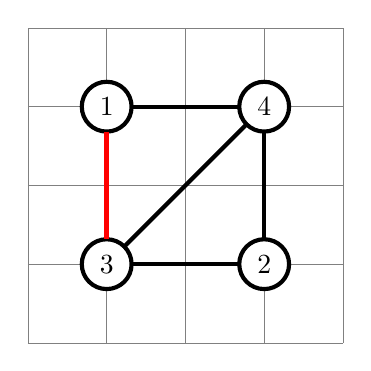
\begin{tikzpicture}
			\draw[help lines] (0,0) grid (4,4);
			%\GraphInit[vstyle=Normal]
			\SetVertexNormal[
			Shape 		= circle,
			LineWidth 	= 1.5pt]
			\SetUpEdge[
			lw 		= 1.5pt,
			color 	= black]
			
			\Vertex[x=1, y=1]{3}
			\Vertex[x=1, y=3]{1}
			\Vertex[x=3, y=1]{2}
			\Vertex[x=3, y=3]{4}
			
			\Edges(3,4)
			\Edges(3,2)
			\Edges[color=red, lw = 2pt](1,3)
			\Edges(2,4)
			\Edges(1,4)
			\end{tikzpicture}
			
			\pause 
			
			\column{.5\textwidth}
			\begin{block}{Take 1 into VC}
				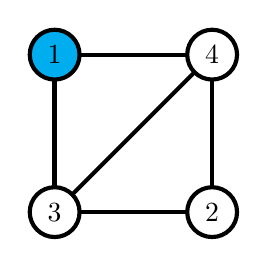
\begin{tikzpicture}
				%\draw[help lines] (0,0) grid (4,2);
				\GraphInit[vstyle=Normal]
				\SetVertexNormal[
				Shape 		= circle,
				LineWidth 	= 1.5pt]
				
				\SetUpEdge[
				lw 		= 1.5pt,
				color 	= black]
				
				\Vertex[x=1, y=1]{3}
				{\renewcommand{\VertexLightFillColor}{cyan} \Vertex[x=1, y=3]{1}}
				\Vertex[x=3, y=1]{2}
				\Vertex[x=3, y=3]{4}
				

				
				\Edges(3,4)
				\Edges(3,2)
				\Edges[lw = 2pt](1,3)
				\Edges(2,4)
				\Edges(1,4)
				\end{tikzpicture}
			\end{block}
		
			\begin{block}{Take 3 into VC}
				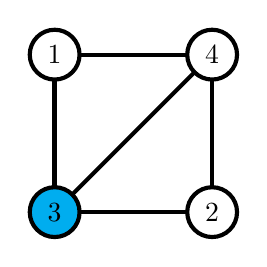
\begin{tikzpicture}
				%\draw[help lines] (0,0) grid (4,2);
				\GraphInit[vstyle=Normal]
				\SetVertexNormal[
				Shape 		= circle,
				LineWidth 	= 1.5pt]
				\SetUpEdge[
				lw 		= 1.5pt,
				color 	= black]
				
				{\renewcommand{\VertexLightFillColor}{cyan} \Vertex[x=1, y=1]{3}}
				\Vertex[x=1, y=3]{1}
				\Vertex[x=3, y=1]{2}
				\Vertex[x=3, y=3]{4}
				
				\Edges(3,4)
				\Edges(3,2)
				\Edges[lw = 2pt](1,3)
				\Edges(2,4)
				\Edges(1,4)
				\end{tikzpicture}
			\end{block}
		\end{columns}
	\end{frame}
	
	\begin{frame}
		\frametitle{Neighbour Branching}
		\begin{columns}[c]
			\column{.5\textwidth}
			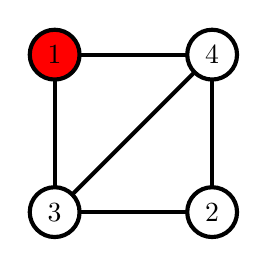
\begin{tikzpicture}
				%\draw[help lines] (0,0) grid (4,4);
				%\GraphInit[vstyle=Normal]
				\SetVertexNormal[
				Shape 		= circle,
				LineWidth 	= 1.5pt]
				\SetUpEdge[
				lw 		= 1.5pt,
				color 	= black]
				
				\Vertex[x=1, y=1]{3}
				{\renewcommand{\VertexLightFillColor}{red} \Vertex[x=1, y=3]{1}}
				\Vertex[x=3, y=1]{2}
				\Vertex[x=3, y=3]{4}
				
				\Edges(3,4)
				\Edges(3,2)
				\Edges(1,3)
				\Edges(2,4)
				\Edges(1,4)
			\end{tikzpicture}
			
			\pause 
			
			\column{.5\textwidth}
			\begin{block}{Take 1 into VC}
				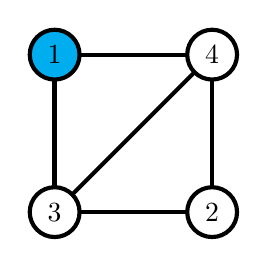
\begin{tikzpicture}
				%\draw[help lines] (0,0) grid (4,2);
				\GraphInit[vstyle=Normal]
				\SetVertexNormal[
				Shape 		= circle,
				LineWidth 	= 1.5pt]
				
				\SetUpEdge[
				lw 		= 1.5pt,
				color 	= black]
				
				\Vertex[x=1, y=1]{3}
				{\renewcommand{\VertexLightFillColor}{cyan} \Vertex[x=1, y=3]{1}}
				\Vertex[x=3, y=1]{2}
				\Vertex[x=3, y=3]{4}
				
				\Edges(3,4)
				\Edges(3,2)
				\Edges[lw = 2pt](1,3)
				\Edges(2,4)
				\Edges(1,4)
				\end{tikzpicture}
			\end{block}
	
			\begin{block}{Take N(1) into VC}
				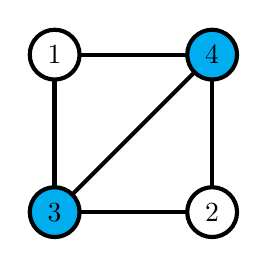
\begin{tikzpicture}
				%\draw[help lines] (0,0) grid (4,2);
				\GraphInit[vstyle=Normal]
				\SetVertexNormal[
				Shape 		= circle,
				LineWidth 	= 1.5pt]
				\SetUpEdge[
				lw 		= 1.5pt,
				color 	= black]
				
				\Vertex[x=1, y=3]{1}
				\Vertex[x=3, y=1]{2}
				{\renewcommand{\VertexLightFillColor}{cyan} \Vertex[x=3, y=3]{4} \Vertex[x=1, y=1]{3}}
				
				\Edges(3,4)
				\Edges(3,2)
				\Edges[lw = 2pt](1,3)
				\Edges(2,4)
				\Edges(1,4)
				\end{tikzpicture}
			\end{block}
		\end{columns}	
	\end{frame}

	\begin{frame}
		\frametitle{Max Degree Selection}
		\begin{columns}[c]
			\column{.5\textwidth}
			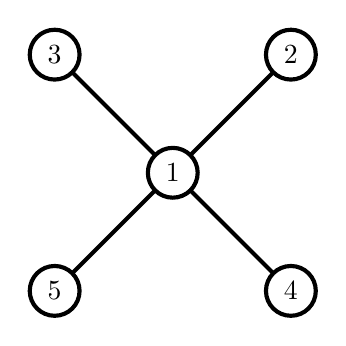
\begin{tikzpicture}
				%\draw[help lines] (0,0) grid (4,4);
				%\GraphInit[vstyle=Normal]
				\SetGraphUnit{1.5}
				\SetVertexNormal[
				Shape 		= circle,
				LineWidth 	= 1.5pt]
				\SetUpEdge[
				lw 		= 1.5pt,
				color 	= black]
				
				\Vertex{1}
				\NOEA(1){2}
				\NOWE(1){3}
				\SOEA(1){4}
				\SOWE(1){5}
				\foreach \v in {2,3,4,5}{\Edge(1)(\v)};
			\end{tikzpicture}
			
			\pause
			\column{.5\textwidth}
			\begin{block}{Random Selection}
				\hspace{0.9cm}
				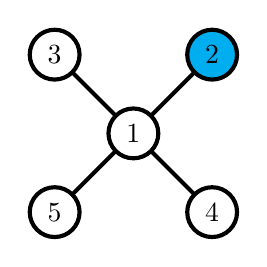
\begin{tikzpicture}
					%\draw[help lines] (0,0) grid (4,2);
					\SetVertexNormal[
					Shape 		= circle,
					LineWidth 	= 1.5pt]
					
					\SetUpEdge[
					lw 		= 1.5pt,
					color 	= black]
					
					\Vertex{1}
					{\renewcommand{\VertexLightFillColor}{cyan} \NOEA(1){2}}
					\NOWE(1){3}
					\SOEA(1){4}
					\SOWE(1){5}
					\foreach \v in {2,3,4,5}{\Edge(1)(\v)};
				\end{tikzpicture}
			\end{block}
			
			
			\begin{block}{Max Degree Selection}
				\hspace{0.9cm}
				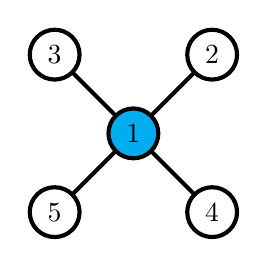
\begin{tikzpicture}
					%\draw[help lines] (0,0) grid (4,2);
					\SetVertexNormal[
					Shape 		= circle,
					LineWidth 	= 1.5pt]
					\SetUpEdge[
					lw 		= 1.5pt,
					color 	= black]
					
					{\renewcommand{\VertexLightFillColor}{cyan} \Vertex{1}}
					\NOEA(1){2}
					\NOWE(1){3}
					\SOEA(1){4}
					\SOWE(1){5}
					\foreach \v in {2,3,4,5}{\Edge(1)(\v)};
				\end{tikzpicture}
			\end{block}
		\end{columns}	
	\end{frame}
	
	\begin{frame}
		\frametitle{Edge Branching Results}
		\begin{figure}
			\begin{tikzpicture}
			\begin{axis}[
				width=1\textwidth,
				height=0.55\textwidth,
				xlabel=k,
				ylabel=seconds]
				\addplot[only marks,color=black,mark=+] table[x={k}, y={time}, col sep=comma] {edge_benchmark.csv};
			\end{axis}
			\end{tikzpicture}
		\end{figure}
	\end{frame}
	
	\begin{frame}
		\frametitle{Neighbour Branching Results}
		\begin{figure}
			\begin{tikzpicture}
				\begin{axis}[
					width=1\textwidth,
					height=0.55\textwidth,
					xlabel=k,
					ylabel=seconds]
					\addplot[only marks,color=black,mark=+] table[x={k}, y={time}, col sep=comma] {neighbour_benchmark.csv};
				\end{axis}
			\end{tikzpicture}
		\end{figure}
	\end{frame}
	
	\begin{frame}[fragile]
		\frametitle{Degree distribution}	
		\begin{figure}
			\begin{tikzpicture}
				\begin{axis}[
					title=Graph on 150 vertices,
					width=1\textwidth,
					height=0.55\textwidth,
					symbolic x coords = {1,2,3,4,5,6,7,8,9,10+},
					ybar,
					xtick=data]
					\addplot table[x={degree}, y={vertices}, col sep=comma] {degrees150.csv};
				\end{axis}
			\end{tikzpicture}
		\end{figure}
\end{frame}

	\begin{frame}[fragile]
		\frametitle{Degree distribution}
		\begin{figure}
			\begin{tikzpicture}
			\begin{axis}[
				title=Graph on 195 vertices,
				width=1\textwidth,
				height=0.55\textwidth,
				symbolic x coords = {1,2,3,4,5,6,7,8,9,10,11,12,13,14,15,16,17,18,19},
				ybar]
				\addplot table[x={degree}, y={vertices}, col sep=comma] {degrees195.csv};
			\end{axis}
			\end{tikzpicture}
		\end{figure}
\end{frame}

	\begin{frame}[fragile]	
		\frametitle{Degree distribution}
		\begin{figure}
			\begin{tikzpicture}
			\begin{axis}[
			title=Graph on 1000 vertices,
			ymode=log,
			log ticks with fixed point,
			width=1\textwidth,
			height=0.55\textwidth,
			ybar,
			bar width=1.2,
			ymin=0,
			xtick={0,10,20,...,90}]
			
			\addplot table[x={degree}, y={vertices}, col sep=comma] {degrees1000.csv};
			\end{axis}
			\end{tikzpicture}
		\end{figure}
\end{frame}
	
	\begin{frame}[plain]
		\centering
		\Large Questions?
	\end{frame}
\end{document}